\subsection{Kortslutningssikring}
\label{effekt_kortslutningssikring}
Kortslutningssikringen tilføjes ved at indføre kredsløbet, vist på figur \ref{fig:dia-kortslut}, mellem base og emitter på darlingtontransistorerne, belastningen og tilbagekoblingen, som vist på figur \ref{fig:dia-kortslut1}. 

\begin{figure}[h]
\centering
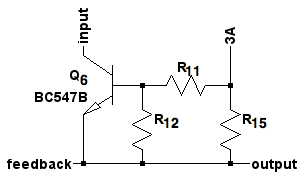
\includegraphics[scale=0.5]{teknisk/effektforstaerker/diagram-kortslut.png}
\caption{Overordnet diagram over kortslutningssikringens aktiveringssituation}
\label{fig:dia-kortslut}
\end{figure}

Strømmen på 3 A, anført på figur \ref{fig:dia-kortslut}, er den strøm, hvor kortslutningssikringen skal aktivere, hvilket blev bestemt i afsnit \ref{valg_kortslutningssikring}. At kortslutningssikringen skal aktivere betyder her, at transistoren Q1 skal åbnes. Når transistoren, Q1, åbnes vil den trække en strøm, hvormed strømmen ind i darlingtontransistorens base går mod nul og darlingtontransistoren lukker. 

\begin{figure}[h]
\centering
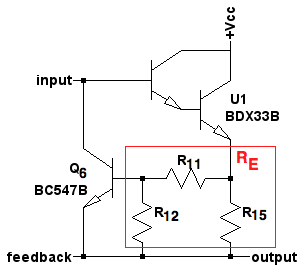
\includegraphics[scale=0.5]{teknisk/effektforstaerker/diagram-kortslut1.png}
\caption{Overordnet diagram over kortslutningssikring forbundet darlingtontransistor}
\label{fig:dia-kortslut1}
\end{figure}

Modstandene $R_1$, $R_2$ og $R_3$ skal, som vist på figur \ref{fig:dia-kortslut1}, repræsentere samme modstandsværdi som $R_E$, som blev beregnet i afsnit \ref{effekt_stroemforstaerker}, da den stadig skal sikre termisk stabilitet. For at åbne Q1 skal der, ifølge databladet for en BC547B \cite{bc547b-datablad}, være en base-emitter spænding på 720 mV \fixme{Jonas- Åbner den ikke lidt før?}, hvilket vil sige spændingen over $R_3$ skal være 720 mV når der løber 3 A fra darlingtontransistorens emitter. Dermed er det muligt at opstille de to udtryk vist formel (\ref{equ:kortslut-betingelse}) og i formel (\ref{equ:kortslut-betingelse1}) til bestemmelse af de tre modstande.

\begin{equation}
\label{equ:kortslut-betingelse}
\mathrm{536~m\ohm} = \frac{1}{\frac{1}{R_1}+\frac{1}{R_2 + R_3}}
\end{equation}

\begin{equation}
\label{equ:kortslut-betingelse1}
\mathrm{720~mV} = R_3 \cdot \frac{R_1 \cdot \mathrm{3~A}}{R_ 1+ R_2 + R_3}
\end{equation}

Det vides desuden, at modstanden af en parallelkobling af modstande er mindre end modstanden af den mindste gren i parallelkoblingen. Dermed vælges $R_1$ til den mindste tilgængelige effektmodstand, som er større end den beregnede $R_E$ modstand. Størrelsen på $R_1$ er derfor 0,68~\ohm, hvorved $R_2$ og $R_3$ kan bestemmes til henholdsvis 1,40~\ohm~ og 1,13~\ohm. Effekten afsat i en modstand kan bestemmes som $P = I^2 \cdot R$, hvorved effekten afsat i hver enkelt af de tre modstande $R_1$, $R_2$ og $R_3$ kan bestemmes som vist i henholdsvis formel (\ref{equ:pr1}), formel (\ref{equ:pr2}) og formel (\ref{equ:pr3}).

\begin{equation}
\label{equ:pr1}
P_{R_1} = \left(\frac{(R_2 + R_3) \cdot \mathrm{3~A}}{R_1 + R_2 + R_3}\right)^2 \cdot R_1 = \mathrm{3,80~W}
\end{equation}

\begin{equation}
\label{equ:pr2}
P_{R_2} = \left(\frac{R_1 \cdot \mathrm{3~A}}{R_1 + R_2 + R_3}\right)^2 \cdot R_2 = \mathrm{0,56~W}
\end{equation}

\begin{equation}
\label{equ:pr3}
P_{R_3} = \left(\frac{R_1 \cdot \mathrm{3~A}}{R_1 + R_2 + R_3}\right)^2 \cdot R_3 = \mathrm{0,47~W}
\end{equation}

Da de tilgængelige effektmodstande kan holde til, at der afsættes en effekt på ??\fixme{Hvad, Frede?} W i dem kontinuerligt, betyder det, at det ikke er nødvendigt at gøre noget for at sikre dem. Alle udregninger i dette afsnit \ref{effekt_kortslutningssikring} er desuden under antagelse af, at strømmen ind i basen på transistoren, Q1, er ubetydelig lille.\\
Her er desuden kun vist for den halvdel af udgangstrinnet som håndterer den positive halvperiode af signalet, der skal dog indføres næsten samme kredsløb på den halvdel som håndterer den negative halvperiode af signalet. Eneste forskel er at transistoren, Q1, erstattes med en BC557B \cite{bc557b-datablad}. Dette gøres da en BC547B vil blive forspændt over base-collector diodeovergangen, hvorved den vil stjæle basestrømmen fra udgangstransistoren. Skulle dette få lov til at ske, vil den negative halvperiode af signalet blive klippet, hvilket ikke vil være tilfældet når der benyttes en BC557B i kortslutningssikringen. 

\subsubsection*{Simulering}